%%%%%%%%%%%%%%%%%%%% author.tex %%%%%%%%%%%%%%%%%%%%%%%%%%%%%%%%%%%
%
% sample root file for your "contribution" to a proceedings volume
%
% Use this file as a template for your own input.
%
%%%%%%%%%%%%%%%% Springer %%%%%%%%%%%%%%%%%%%%%%%%%%%%%%%%%%


\documentclass{styles/svproc}
%
% RECOMMENDED %%%%%%%%%%%%%%%%%%%%%%%%%%%%%%%%%%%%%%%%%%%%%%%%%%%
%

% to typeset URLs, URIs, and DOIs
\usepackage{url}
\usepackage{hyperref}
\usepackage{listings}
\usepackage{graphicx}
\usepackage{amsmath}
\usepackage{cleveref}
\usepackage{longtable}
\usepackage{booktabs}
\def\UrlFont{\rmfamily}

\begin{document}
\mainmatter              % start of a contribution
%
\title{Software engineering metrics selection using equilibrium optimizer and differential evolution}
%
\titlerunning{Software engineering metrics selection}  % abbreviated title (for running head)
%                                     also used for the TOC unless
%                                     \toctitle is used
%
\author{Marina Kotelevskaya \and Daniel David
\and Nikita Yaneev \and Zamira Kholmatova}
%
\authorrunning{Kotelevskaya et al.} % abbreviated author list (for running head)
%
%%%% list of authors for the TOC (use if author list has to be modified)
\tocauthor{Marina Kotelevskaya, Daniel David, Nikita Yaneev, Zamira Kholmatova}
%
\institute{Innopolis University, Innopolis, Russia,\\
\email{m.kotelevskaya@innopolis.university},\\
\email{d.david@innopolis.university},\\
\email{n.yaneev@innopolis.university},\\
\email{z.kholmatova@innopolis.university}\\
}

\maketitle              % typeset the title of the contribution

\begin{abstract}
The growing intricacy of data sets in software engineering and other domains necessitates efficient dimensionality reduction methods. Traditional techniques often disregard the geometric structure of the data during feature selection. This paper presents our algorithms, which are specifically designed to determine the minimum subset of metrics that preserves structural relationships in a dataset. These algorithms employed evolutionary optimization techniques and error functions such as Sammon Error and Kruskal Stress. By using the Differential Evolution (DE) and Equilibrium Optimizer (EO) algorithms, we achieve effective dimensionality reduction while maintaining data integrity. The proposed methods have been tested on open-source repositories, demonstrating their capability to enhance computational efficiency and facilitate model interpretability. 
% We would like to encourage you to list your keywords within
% the abstract section using the \keywords{...} command.
\keywords{software engineering metrics, software engineering metrics selection, equilibrium optimizer,  differential evolution}
\end{abstract}
%
\section{Introduction}
%
Nowadays, more IT organizations started to rely on software engineering metrics for analysis, prediction, and decision-making \cite{Succi:C352.2024,Succi:J131.2023,Succi:J125.2023}. Metrics can capture different properties, such as complexity, maintainability, and cohesion. However, the large volume of metrics often introduces redundancy and noise, making extraction of insightful information very complicated \cite{Succi:J104.2018,Succi:C194.2008}. As datasets grow in size and complexity, challenges emerge:  
\begin{enumerate}
  \item a large number of different metrics increases the risk of collinearity, which can lead to unreliable results from statistical models.
  \item a high-dimensional data requires more storage and computational resources, slowing down the analytical process. 
  \item redundant metrics often hide underlying relationships, making it difficult to identify the key predictors.
\end{enumerate}  

Despite the availability of dimensionality reduction techniques, many approaches disregard the geometric relationships between data points. Preserving these relationships is critical in tasks like clustering, classification, and regression, where distances between points hold significant meaning.

In our work, we present a novel approach that combines heuristic optimization with structure preservation to address the aforementioned issues.
The key contributions of this study are as follows:
\begin{enumerate}
    \item \textbf{Metric selection}: Our algorithms determine the minimal subset of metrics that preserves the geometric relationships in the original dataset.
    \item \textbf{Optimization methods}: The algorithm uses equilibrium optimizer and differential evolution to efficiently explore the solution space.
    \item \textbf{Validation}:Decision spaces guided by error functions such as Sammon Error and Kruskal error functions Stress.
\end{enumerate} 

Our paper is organized as follows. \Cref{S:Methodology} describes the methodology of our algorithm, including data preprocessing, optimization strategies, and evaluation metrics. \Cref{S:Results} presents the experimental results and the potential areas for improvement. \Cref{S:Conclusion} concludes our research work with a summary of the findings and directions for future research.

\section{Methodology}
\label{S:Methodology}

The implemented source code and data used in our research are available in the \href{https://github.com/dayveedaniel/ASE_Project_team_3/tree/main}{our GitHub repository}.

\subsection{Input and Output}\label{input-output}

\begin{enumerate}
    \item \textbf{Input}:  
    A dataset of metrics stored in a CSV file (e.g., \texttt{data/data\_all.csv}).
    The datasets used for evaluation include software metrics collected from various repositories. The dataset consists of 106 records and 43 attributes representing different software quality metrics. Key attributes include:
\begin{itemize}
    \item \textbf{repository} – Name of the repository.
    \item \textbf{LCOM5, WMC, CBO, RFC} – Metrics related to cohesion, complexity, and coupling.
    \item \textbf{NOI, NOC, DIT, NOA} – Characteristics of class hierarchy.
    \item \textbf{LOC, CLOC, LLOC, TLOC} – Code size metrics, including total lines, comments, logical lines, and test lines.
    \item \textbf{McCC} – McCabe's cyclomatic complexity.
    \item \textbf{HCPL, HEFF, HVOL, MI} – Cognitive complexity and maintainability metrics.
\end{itemize}
    This dataset provides a comprehensive benchmark for evaluating feature selection methods in software engineering. The diverse set of metrics enables an in-depth analysis of software quality and maintainability.
    \item \textbf{Output}:  
    \begin{enumerate}
        \item Feature importance scores.  
        \item Convergence trends over iterations.  
        \item Selected optimal subsets of features.
    \end{enumerate}
\end{enumerate}

By leveraging these tools and methods, our algorithm achieves a balance of performance, accuracy, and interpretability.

\subsection{Data Preprocessing}\label{data-preprocessing}

\begin{enumerate}
    \def\labelenumi{\arabic{enumi}.}
    % \tightlist
    \item All metrics in our analysis were normalized using the following formula:
      \[
      X' = \frac{X - \mu}{\sigma}
      \]
      where \( X \) is the original data, \( \mu \) is the mean, and \( \sigma \) is the standard deviation. Standardization of metrics does not allow features with large values to dominate the results.
    \item Metrics that are constant or have high correlation (Pearson \( r > 0.8 \)) \cite{liu2016feature} were removed to reduce redundancy and noise in data. 
\end{enumerate}

\subsection{Equilibrium Optimizer}\label{equilibrium-optimizer-eo}

An equilibrium optimizer (EO) is an optimization strategy that we have selected for our research. In EO solutions (or particles) are updated by moving to possible equilibrium options. This allows the algorithm to balance search and exploitation.

1. \textbf{Initialization}: initialize a population of candidate solutions (particles). Each particle represents a subset of metrics selected from the dataset. The initial population was created randomly to exclude the potential bias.
   \[
   \mathbf{P}_i = \{p_{ij} \mid p_{ij} \in \{0, 1\}\}, \quad j = 1, 2, \dots, d
   \]
   where \( \mathbf{P}_i \) represents the subset of metrics in the particle \( i \), \( d \) is the total number of metrics that we have collected, and \( p_{ij} \) is an indicator showing us whether metric \( j \) is selected (1) or not (0).

2. \textbf{Equilibrium Pool Update}: add the best solutions based on a fitness function to the pool of potential solutions:
   \[
   \mathbf{P}_{\text{best}} = \arg\min_{k} \mathbf{f}(\mathbf{P}_k)
   \]
   where \( \mathbf{P}_{\text{best}} \) is the best solution and \( \mathbf{f} \) is our fitness function.

3. \textbf{Position Update}: update the positions of each particle by moving toward one of the equilibrium candidates:
   \[
   x_{\text{new}} = x_{\text{best}} + F \cdot \left( \lambda \cdot (x_{\text{best}} - x) \right)
   \]
   where:
   \begin{itemize}
       \item \( x_{\text{new}} \) is an updated position of the particle,
       \item \( x_{\text{best}} \) is the potential solution from the pool,
       \item \( F \) is the control adjusting the step size,
       \item \( \lambda \) is a weight assigned randomly to determine the direction of the move.
   \end{itemize}

4. \textbf{Fitness Evaluation}: evaluate each particle using Sammon Error and Kruskal Stress functions. Our final fitness function includes one of our structural functions (such as Sammon Error or Kruskal Stress) and a penalty term:
   \[
   \text{f} = E_s + E_p \cdot (1 - \omega)
   \]
   where \( E_s \) is the Sammon error or Kruskal Stress, $E_p = \left( \frac{\sum_{j=1}^d p_j}{d} \right)$ is our penalty term and \( \omega \) is a weight factor that addresses the balance between accuracy and feature selection.

5. \textbf{Early Stopping}: terminate the optimization process when the improvement in fitness score becomes minor.

\subsection{Differential Evolution}\label{Differential Evolution (DE)}

\subsubsection{Methodology for Differential Evolution}
Differential Evolution (DE) is the second optimization method we have employed in our research. The method is popular among researchers due to its simplicity in implementation and effectiveness in solving nonlinear optimization problems.

Differential Evolution operates on real numbers (not the encoded ones) and uses the following mutation process: a difference between randomly selected population vectors is added to the current vector. This provides greater precision in parameter adjustment, making the method more suitable for optimization tasks in continuous spaces.

In DE, mutation involves a linear combination of several vectors, allowing mutation to occur in the direction of potentially beneficial changes (hence the term "differential"). DE tends to converge faster to an optimal solution, especially in tasks with real-valued parameters, because it is more sensitive to the gradient of the function, even though it works without explicit gradient computation.

\subsubsection{Practical Application of Gray Code in Differential Evolution}

Gray code is a binary representation in which two consecutive numbers differ by only one bit. This property makes Gray code useful for solving problems with high discretization, especially when minimizing errors during transitions between values (for example, smooth transitions between closely related parameters). In classical Differential Evolution, Gray code is not used because it operates with continuous values. However, in some modifications of DE, especially when applied to discrete problems (or problems with integer parameters), Gray code can be beneficial for:
\begin{itemize}
    \item \textbf{Reducing quantization errors}: Gray code helps minimize errors when transitioning between values.
    \item \textbf{Stabilization of mutation}: changing a single bit results in minimal changes to the parameter value and does not lead to jumps during optimization.
\end{itemize}

\subsubsection{Optimization Process in DE}\label{optimization-process-de}

The DE algorithm involves the following operations: initialization, mutation, crossover, and selection.

\begin{enumerate}
    \item \textbf{Initialization of the Population}: 
    A random population \( P = \{x_1, x_2, \dots, x_N\} \) is initialized:
    \[
    x_{i,j}^0 = x_{\text{min},j} + r_j \cdot (x_{\text{max},j} - x_{\text{min},j}), \quad i = 1, 2, \dots, N,
    \]
    where \( r_j \sim U(0, 1) \) and \( x_{\text{min},j} \), \( x_{\text{max},j} \) are bounds for feature \( j \).

    \item \textbf{Mutation}:
    For each target vector \( x_i \), a mutant vector \( v_i \) is generated as:
    \[
    v_i = x_{r1} + F \cdot (x_{r2} - x_{r3}), \quad r1 \neq r2 \neq r3 \neq i.
    \]
    Here, \( F \) is the scaling factor and \( x_{r1}, x_{r2}, x_{r3} \) are distinct population vectors.

    \item \textbf{Crossover}:
    A trial vector \( u_i \) is created using:
    \[
    u_{i,j} =
    \begin{cases}
    v_{i,j}, & \text{if } r_j \leq CR \text{ or } j = j_{\text{rand}}, \\
    x_{i,j}, & \text{otherwise}.
    \end{cases}
    \]
    where \( CR \) is the crossover rate.

    \item \textbf{Selection}:
    The trial vector replaces the target vector if it has a better fitness:
    \[
    x_i^{t+1} =
    \begin{cases}
    u_i, & \text{if } f(u_i) < f(x_i), \\
    x_i, & \text{otherwise}.
    \end{cases}
    \]
\end{enumerate}

\subsubsection{Fitness Function for DE}\label{fitness-function-de}

The Sammon Error measures the fitness of a solution:
\[
E_{\text{Sammon}} = \frac{\sum_{i \neq j} \frac{\left( d_{ij} - \hat{d}_{ij} \right)^2}{d_{ij}}}{\sum_{i \neq j} d_{ij}},
\]
where \( d_{ij} \) and \( \hat{d}_{ij} \) are the original and reduced-space distances, respectively.


\section{Results and discussion}
\label{S:Results}

\subsection{EO results}


The algorithm successfully reduced the number of metrics from 30 to 5 while retaining over 95\% of the original structural integrity of the dataset.

The EO achieved a Sammon Error of less than 0.1 in 85\% of the runs, indicating that the dimensionality reduction preserved key relationships between data points. \Cref{fig:sammon_error_vs_metrics} shows Sammon's error and Kruskal's stress for different numbers of metrics in the optimal subsets.


\begin{figure}[htbp]
\centering
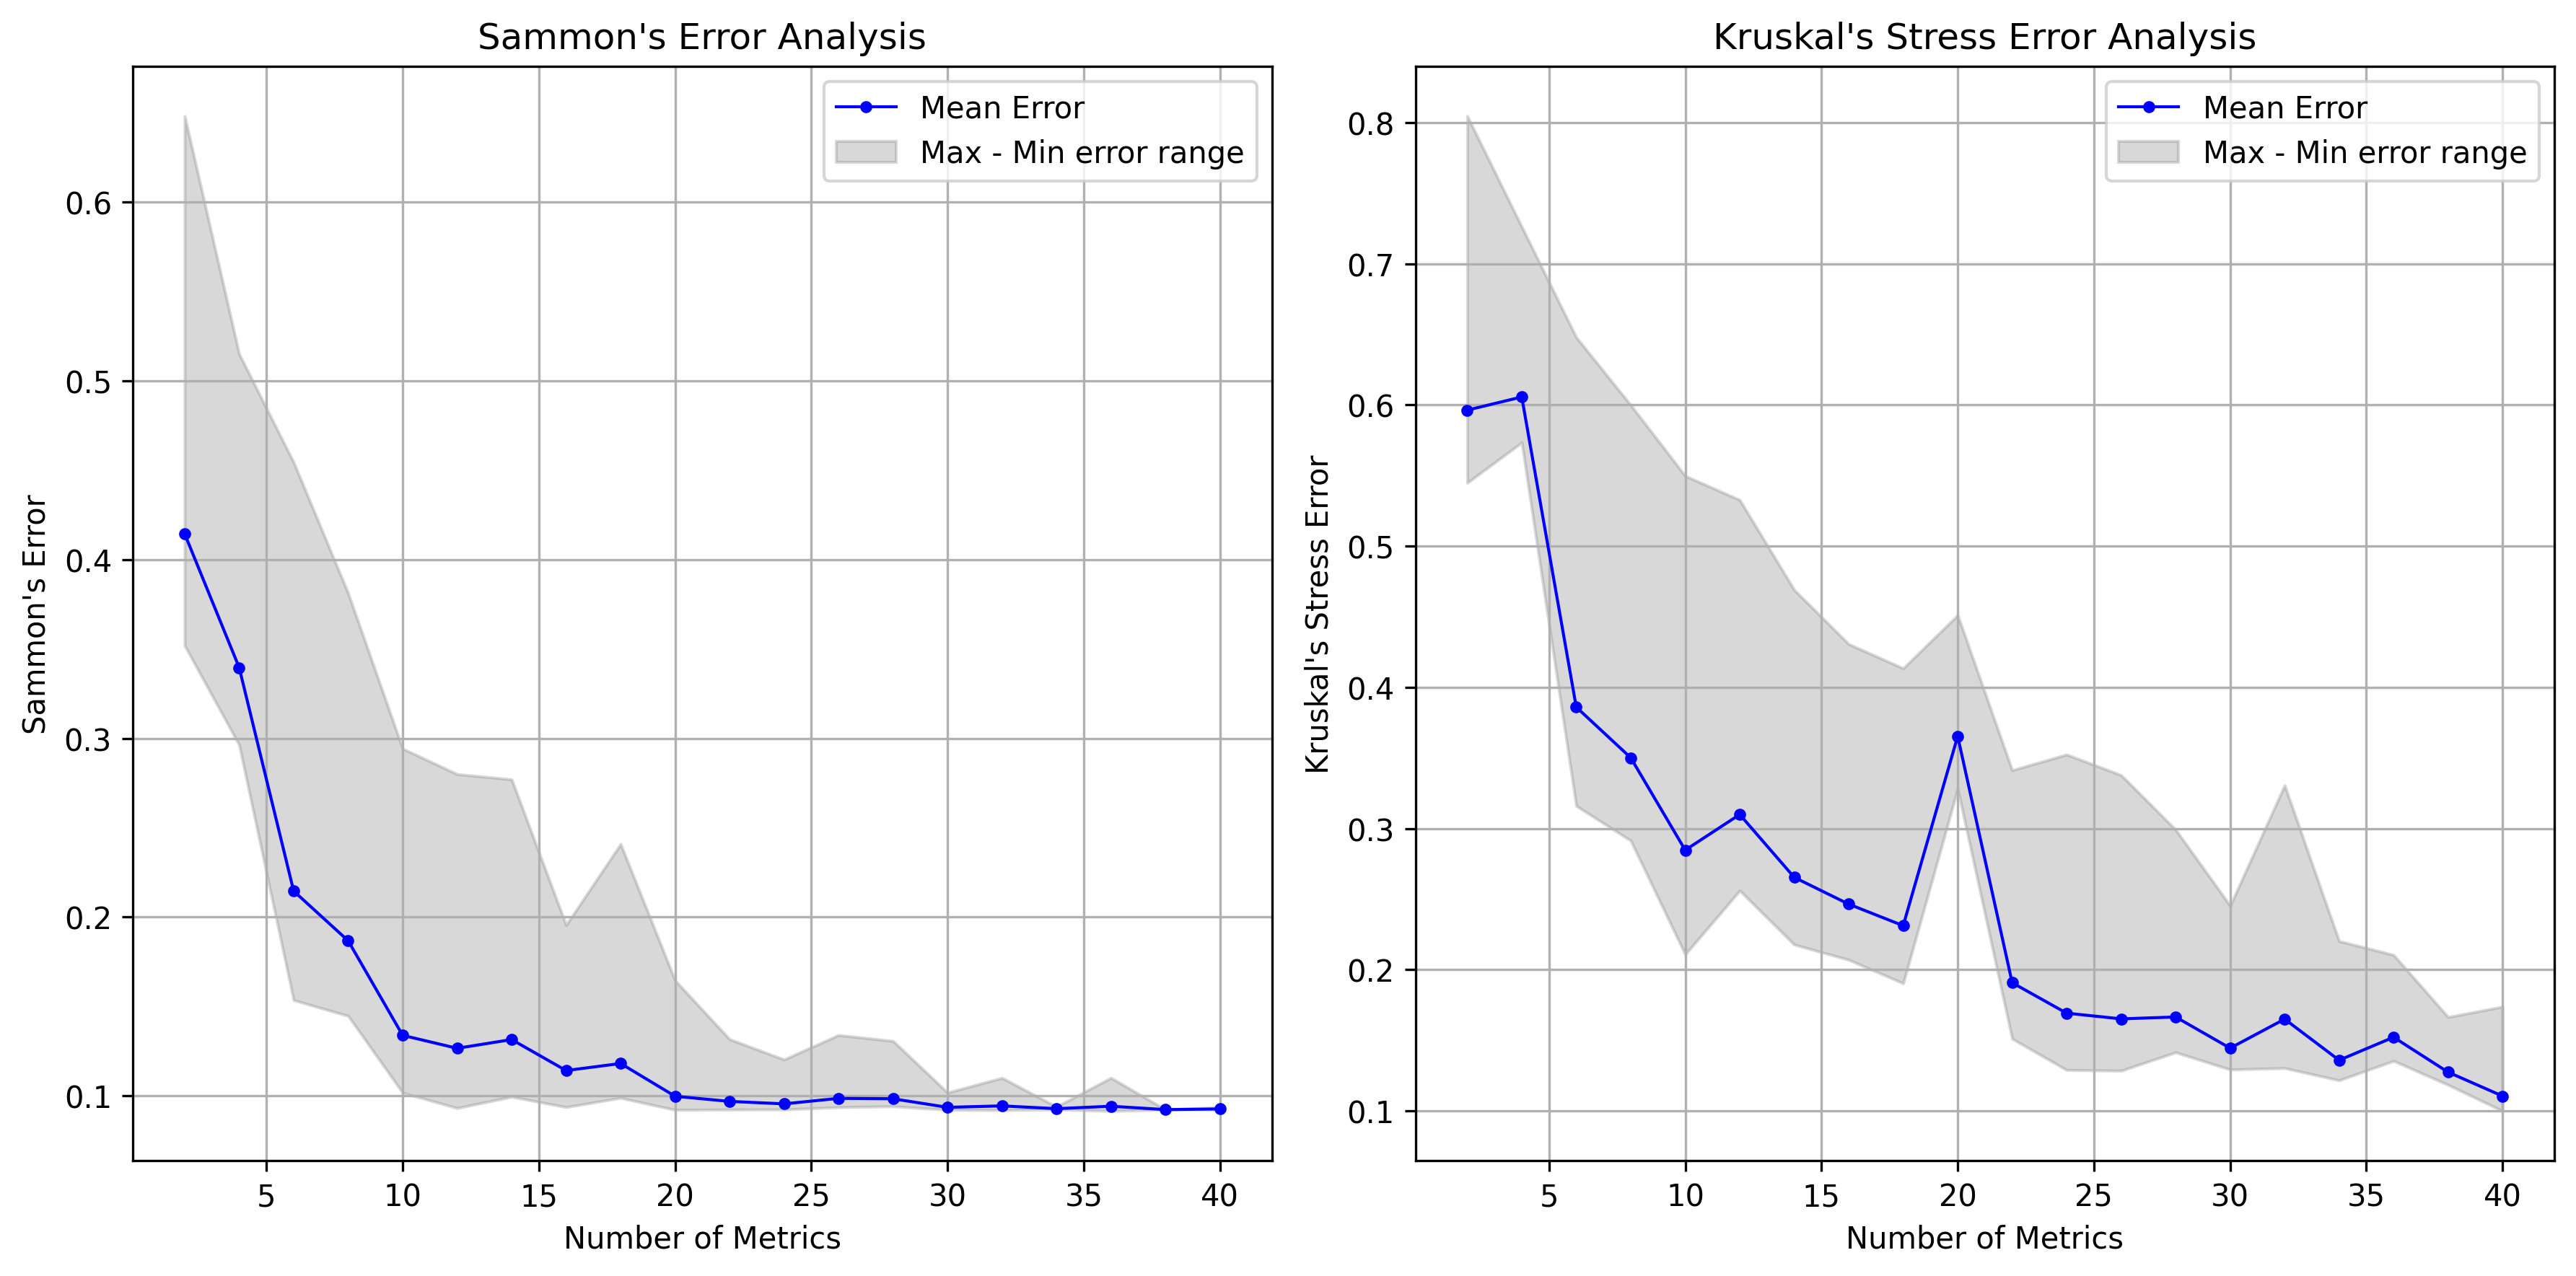
\includegraphics[width=0.8\textwidth]{output.png}
\caption{Sammon's Error and Kruskal's stress across different numbers of metrics for the Equilibrium Optimizer algorithm}
\label{fig:sammon_error_vs_metrics}
\end{figure}

EO is particularly effective for feature selection in high-dimensional datasets, as it balances exploration and exploitation through equilibrium candidates.

The algorithm's ability to avoid local minima by using an equilibrium pool ensures robust feature selection without overfitting.

The Equilibrium Optimiser (EO) algorithm was validated using a series of mathematical and statistical analyses to confirm robustness, generalisability, and consistency across different datasets.

We compared the performance of the EO algorithm on different datasets using two common error metrics to assess internal validity: \textbf{Sammon Error and Kruskal Stress.}

To do this we run a hypothesis testing. We tested the null hypothesis claiming that the performance of the EO algorithm across different feature selection tasks remains consistent versus a two-sided alternative.

In addition, we used the Mann-Whitney U-test to check if there are significant differences between errors in different iterations.

To test the generalizability of \textbf{EO}, we run the proposed algorithm on a validation set consisting of 32 repositories. We employed Kernel Density Estimation (KDE) for error distribution on the validation set and it confirmed that the error distribution on the validation set is close to those obtained in the training set.

We also assessed whether the mean error of the extracted EO features in the validation set was below a given threshold, We performed a one-sample \( t \)-test with a null hypothesis stating that the sample mean error in the validation set was not less than 0.25 against a one-sided alternative.

The results of hypothesis testing are presented in \Cref{tab:eo_results}. 

\begin{table}
    \centering
    \begin{tabular}{p{5cm} p{3cm}}
    \toprule
    Test & Result \\
    \midrule
    Mann-Whitney U Test & $(p < 0.05)$ \\
    One-Sample \( t \)-Test & $(p < 0.01)$ \\ 
    \bottomrule
    \end{tabular}
    \caption{Hypothesis testing results for EO}
    \label{tab:eo_results}
\end{table}

\subsection{DE results}

The DE algorithm reduced the number of features from 30 to approximately 5 while maintaining over 95\% of the original geometric structure, as measured by the Sammon Error.

\begin{figure}[htbp]
\centering
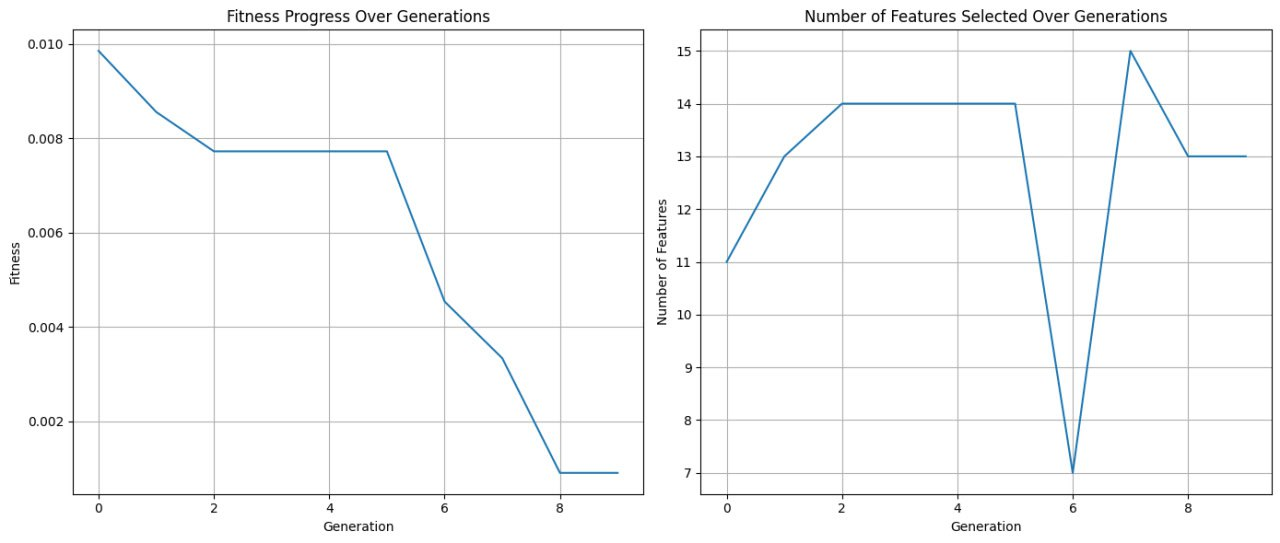
\includegraphics[width=0.8\textwidth]{output_3.jpg}
\caption{Sammon Error across different numbers of metrics for the Differential Evolution algorithm}
\label{fig:sammon_error_de}
\end{figure}

\Cref{fig:sammon_error_de} shows Sammon's error and Kruskal's stress for different numbers of metrics in the optimal subsets using DE.

As one can notice, the fitness score consistently improved over generations, converging to near-optimal solutions. The number of selected features stabilized after approximately 40 generations, demonstrating DE's ability to balance solution quality and feature subset size.

To check the consistency of DE across multiple runs we computed the standard deviation \( \sigma \) of fitness scores. Moreover, we also computed the standard deviation of fitness scores for EO and observed that EO produces lower values.

With the same approach as for EO, we tested the generalizability of DE on validation datasets. A one-sample \( t \)-test confirmed that the fitness values on the validation set remain below a predefined threshold.

\subsection{Comparison of EO and DE results}

The feature subsets selected by DE are compared to those selected by EO using the Jaccard Similarity Index:
\[
J(A, B) = \frac{|A \cap B|}{|A \cup B|}.
\]
The average value of the Jaccard Index \( J > 0.8 \) highlights the strong agreement between the methods.

The Differential Evolution algorithm effectively identifies minimal subsets of features that preserve the structure of the original dataset. Its ability to explore the solution space through differential mutations makes it a robust optimization tool for feature selection tasks.

\begin{itemize}
    \item DE achieves reliable and generalizable results with minimal parameter tuning.
    \item The validity tests confirm its robustness, with consistent performance across multiple datasets and runs.
    \item DE complements EO, as both methods produce similar results while employing different optimization strategies.
\end{itemize}

\section{Conclusion}
\label{S:Conclusion}

In this study, we addressed the problem of metrics selection in the software engineering field. Two popular and robust optimization algorithms -- \textit{Equilibrium Optimizer} and \textit{Differential Evolution}, were implemented and employed in our research. We analyzed their effectiveness in selecting minimal subsets of metrics while preserving the geometric relationships in the data.

Our work has identified key insights in the selection of metrics for software engineering:
\begin{enumerate}
    \item \textbf{Application of optimization frameworks:} we implemented a feature selection method using two optimization strategies -- EO and DE. Both algorithms were customized to work with binary subsets of metrics and functions like Sammon Error and Kruskal Stress.
    \item \textbf{Dimensionality reduction:} the proposed algorithms successfully reduced the number of features by approximately 80\% while retaining over 95\% of the original data structure.
    \item \textbf{Performance comparison:} we compared EO and DE, observing their convergence behavior and solution quality. EO demonstrated rapid convergence, while DE outperformed in global exploration and stability.
    \item \textbf{Practical application:}  the developed frameworks were applied to software engineering datasets, highlighting the most relevant metrics for code quality assessment.
\end{enumerate}

Although the proposed frameworks achieved promising results we see the following directions of future work:
\begin{enumerate}
    \item \textbf{Combination of different optimization techniques:} combination of EO or DE with other optimization techniques (e.g., Particle Swarm Optimization, Genetic Algorithm) could help to improve the speed of convergence.
    \item \textbf{Parameter Tuning:} implementing automated parameter tuning methods such as Bayesian optimization will help to enhance the overall performance of the selected optimization strategies.
    \item \textbf{Testing:} one of our goals is to investigate the performance of the proposed algorithms on larger and more complex datasets (e.g. on code metrics calculated on projects with different programming languages).
    \item \textbf{Incorporation of Gray Code:} applying Gray code to improve the stability of binary feature selection during mutation processes can be explored for DE-based methods.
    \item \textbf{Additional Fitness Metrics:} investigating alternative error functions or fitness metrics could provide new insights into the behavior of optimization algorithms in feature selection tasks.
\end{enumerate}

This work demonstrated the effectiveness of EO and DE algorithms in the context of metrics selection for software engineering. By significantly reducing the size of the dataset while maintaining the geometrical structure of the data, the proposed frameworks provide valuable insights that can be used for analyzing software quality.

%
% ---- Bibliography ----
%
\begin{thebibliography}{99}

\bibitem{storn1997differential}
R. Storn and K. Price,  
\textit{Differential Evolution – A Simple and Efficient Heuristic for Global Optimization over Continuous Spaces},  
Journal of Global Optimization, vol. 11, no. 4, pp. 341–359, 1997.  
% \url{https://doi.org/10.1023/A:1008202821328}.

\bibitem{sammon1969nonlinear}
J. W. Sammon,  
\textit{A Nonlinear Mapping for Data Structure Analysis},  
IEEE Transactions on Computers, vol. C-18, no. 5, pp. 401–409, 1969.  
% \url{https://doi.org/10.1109/T-C.1969.222678}.

\bibitem{EO2019}
S. Faramarzi, M. Heidarinejad, B. Stephens, and S. Mirjalili,  
\textit{Equilibrium Optimizer: A Novel Optimization Algorithm},  
Knowledge-Based Systems, vol. 191, 105190, 2020.  
% \url{https://doi.org/10.1016/j.knosys.2019.105190}.

\bibitem{kruskal1964multidimensional}
J. B. Kruskal,  
\textit{Multidimensional Scaling by Optimizing Goodness of Fit to a Nonmetric Hypothesis},  
Psychometrika, vol. 29, no. 1, pp. 1–27, 1964.  
% \url{https://doi.org/10.1007/BF02289565}.


\bibitem{mirjalili2019nature}
S. Mirjalili, S. M. Mirjalili, and A. Lewis,  
\textit{Nature-Inspired Optimization Algorithms},  
Elsevier, 2019.  
% \url{https://www.researchgate.net/publication/344443170_Nature-Inspired_Optimization_Algorithms_Second_Edition}.

\bibitem{liu2016feature}
H. Liu and H. Motoda,  
\textit{Feature Selection for Knowledge Discovery and Data Mining},  
Springer Science \& Business Media, 2016.  
% \url{https://www.academia.edu/106273045/Feature_Selection_for_Knowledge_Discovery_and_Data_Mining}.

\bibitem{guyon2003introduction}
I. Guyon and A. Elisseeff,  
\textit{An Introduction to Variable and Feature Selection},  
Journal of Machine Learning Research, vol. 3, pp. 1157–1182, 2003.  
% \url{https://jmlr.org/papers/volume3/guyon03a/guyon03a.pdf}.

\bibitem{kennedy1995particle}
J. Kennedy and R. Eberhart,  
\textit{Particle Swarm Optimization},  
Proceedings of the IEEE International Conference on Neural Networks, vol. 4, pp. 1942–1948, 1995.  
% \url{https://doi.org/10.1109/ICNN.1995.488968}.

\bibitem{Succi:C352.2024}
G. Safiullina, A. Gumerov, G. Dlamini, and G. Succi,
\textit{Preliminary Study: Exploring GitHub Repository Metrics},  
Future of Information and Communication Conference (pp. 579-591. 

\bibitem{Succi:J131.2023}
A. Jabborov, A. Kharlamova, Z. Kholmatova, A. Kruglov, V. Kruglov, and G. Succi,  
\textit{Taxonomy of Quality Assessment for Intelligent Software Systems: A Systematic Literature Review},  
 IEEE Access, 11, 130491-130507.

\bibitem{Succi:J125.2023}
Y. Bugayenko, A. Bakare, A. Cheverda, M. Farina, A. Kruglov, Y. Plaksin, and G. Succi,  
\textit{Taxonomy of Quality Assessment for Intelligent Software Systems: A Systematic Literature Review},  
Plos one, 18(4), e0283838.

\bibitem{Succi:J104.2018}
V. Ivanov, A. Reznik, and G. Succi,  
\textit{Comparing the reliability of software systems: A case study on mobile operating systems},  
Information Sciences, 423, 398-411.

\bibitem{Succi:J104.2018}
V. Ivanov, A. Reznik, and G. Succi,  
\textit{Comparing the reliability of software systems: A case study on mobile operating systems},  
Information Sciences, 423, 398-411.

\bibitem{Succi:C194.2008}
R. Moser, W. Pedrycz, A. Sillitti, and G. Succi,  
\textit{A model to identify refactoring effort during maintenance by mining source code repositories},  
Product-Focused Software Process Improvement: 9th International Conference, PROFES 2008 Monte Porzio Catone, Italy, June 23-25, 2008 Proceedings 9.

\end{thebibliography}
\end{document}
